% Created 2021-04-29 Thu 06:52
% Intended LaTeX compiler: pdflatex
\documentclass[presentation]{beamer}
\usepackage[utf8]{inputenc}
\usepackage[T1]{fontenc}
\usepackage{graphicx}
\usepackage{grffile}
\usepackage{longtable}
\usepackage{wrapfig}
\usepackage{rotating}
\usepackage[normalem]{ulem}
\usepackage{amsmath}
\usepackage{textcomp}
\usepackage{amssymb}
\usepackage{capt-of}
\usepackage{hyperref}
\RequirePackage{fancyvrb}
\DefineVerbatimEnvironment{verbatim}{Verbatim}{fontsize=\scriptsize}
\usetheme{metropolis}
\usecolortheme{}
\usefonttheme{}
\useinnertheme{}
\useoutertheme{}
\author{Petru Rebeja, Marius Apetrii}
\date{29 Aprilie 2021}
\title{Tehnici Avansate de Programare}
\subtitle{ASP.NET Core MVC --- Introducere}
\institute[UAIC]{Facultatea de Matematică\\Universitatea Alexandru Ioan Cuza, Iași}
\hypersetup{
 pdfauthor={Petru Rebeja, Marius Apetrii},
 pdftitle={Tehnici Avansate de Programare},
 pdfkeywords={},
 pdfsubject={},
 pdfcreator={Emacs 26.3 (Org mode 9.4.4)},
 pdflang={Romanian}}
\begin{document}

\maketitle
\section{Introducere}
\label{sec:orgfc078e0}
\begin{frame}[label={sec:orge24cdc4}]{Recapitulare}
\pause
\begin{itemize}
\item \alert{Baza de date} este o colecție organizată de date care pot fi manipulate prin intermediul unui \alert{Sistem de Gestiune al Bazelor de Date}.
\end{itemize}
\pause
\begin{itemize}
\item \alert{Schema bazei de date} este reprezentarea structurii bazei de date. Visual Studio ne pune la dispoziţie un şablon de proiect pentru păstrarea şi modificarea schemei.
\end{itemize}
\pause
\begin{itemize}
\item Bazele de date relaţionale pun accentul pe proprietățile \alert{ACID}; bazele de date non-relaționale --- teorema \alert{CAP}.
\end{itemize}
\end{frame}
\begin{frame}[label={sec:orga507381},fragile]{Agenda}
 \begin{itemize}
\item Şablonul \texttt{MVC}
\item Introducere în \texttt{ASP.NET Core MVC}
\end{itemize}
\end{frame}
\section{Şablonul \texttt{MVC}}
\label{sec:orgf4cc7b4}
\begin{frame}[label={sec:orgaf6ae93},fragile]{\texttt{Model-View-Controller}}
 \begin{block}{MVC}
\alert{Model-View-Controller} este un şablon de proiectare utilizat pentru a decupla interfaţa grafică (\texttt{view}), datele (\texttt{model}) şi logica aplicaţiei (\texttt{controller})\footnote{\url{https://dotnet.microsoft.com/apps/aspnet/mvc}}.
\end{block}
\end{frame}
\begin{frame}[label={sec:orgb999d76},fragile]{Componente}
 \begin{itemize}
\item \texttt{Modelul} --- încapsulează datele şi logica aplicaţiei; este independent de interfaţa cu utilizatorul\footnote{Burbeck, Steve (1992) Applications Programming in Smalltalk-80:How to use Model–View–Controller (MVC)}.
\item \texttt{Viewul} --- prezintă datele din \texttt{model} în diverse formate; acelaşi \texttt{model} poate avea mai multe \texttt{viewuri}.
\item \texttt{Controllerul} --- converteşte datele de intrare în comenzi pentru \texttt{Model} sau \texttt{View}\footnote{\url{https://www.codeproject.com/Articles/25057/Simple-Example-of-MVC-Model-View-Controller-Design}} şi le validează dacă este nevoie.
\end{itemize}
\end{frame}
\begin{frame}[label={sec:orgaf78339},fragile]{\texttt{Model-View-Controller}}
 \begin{center}
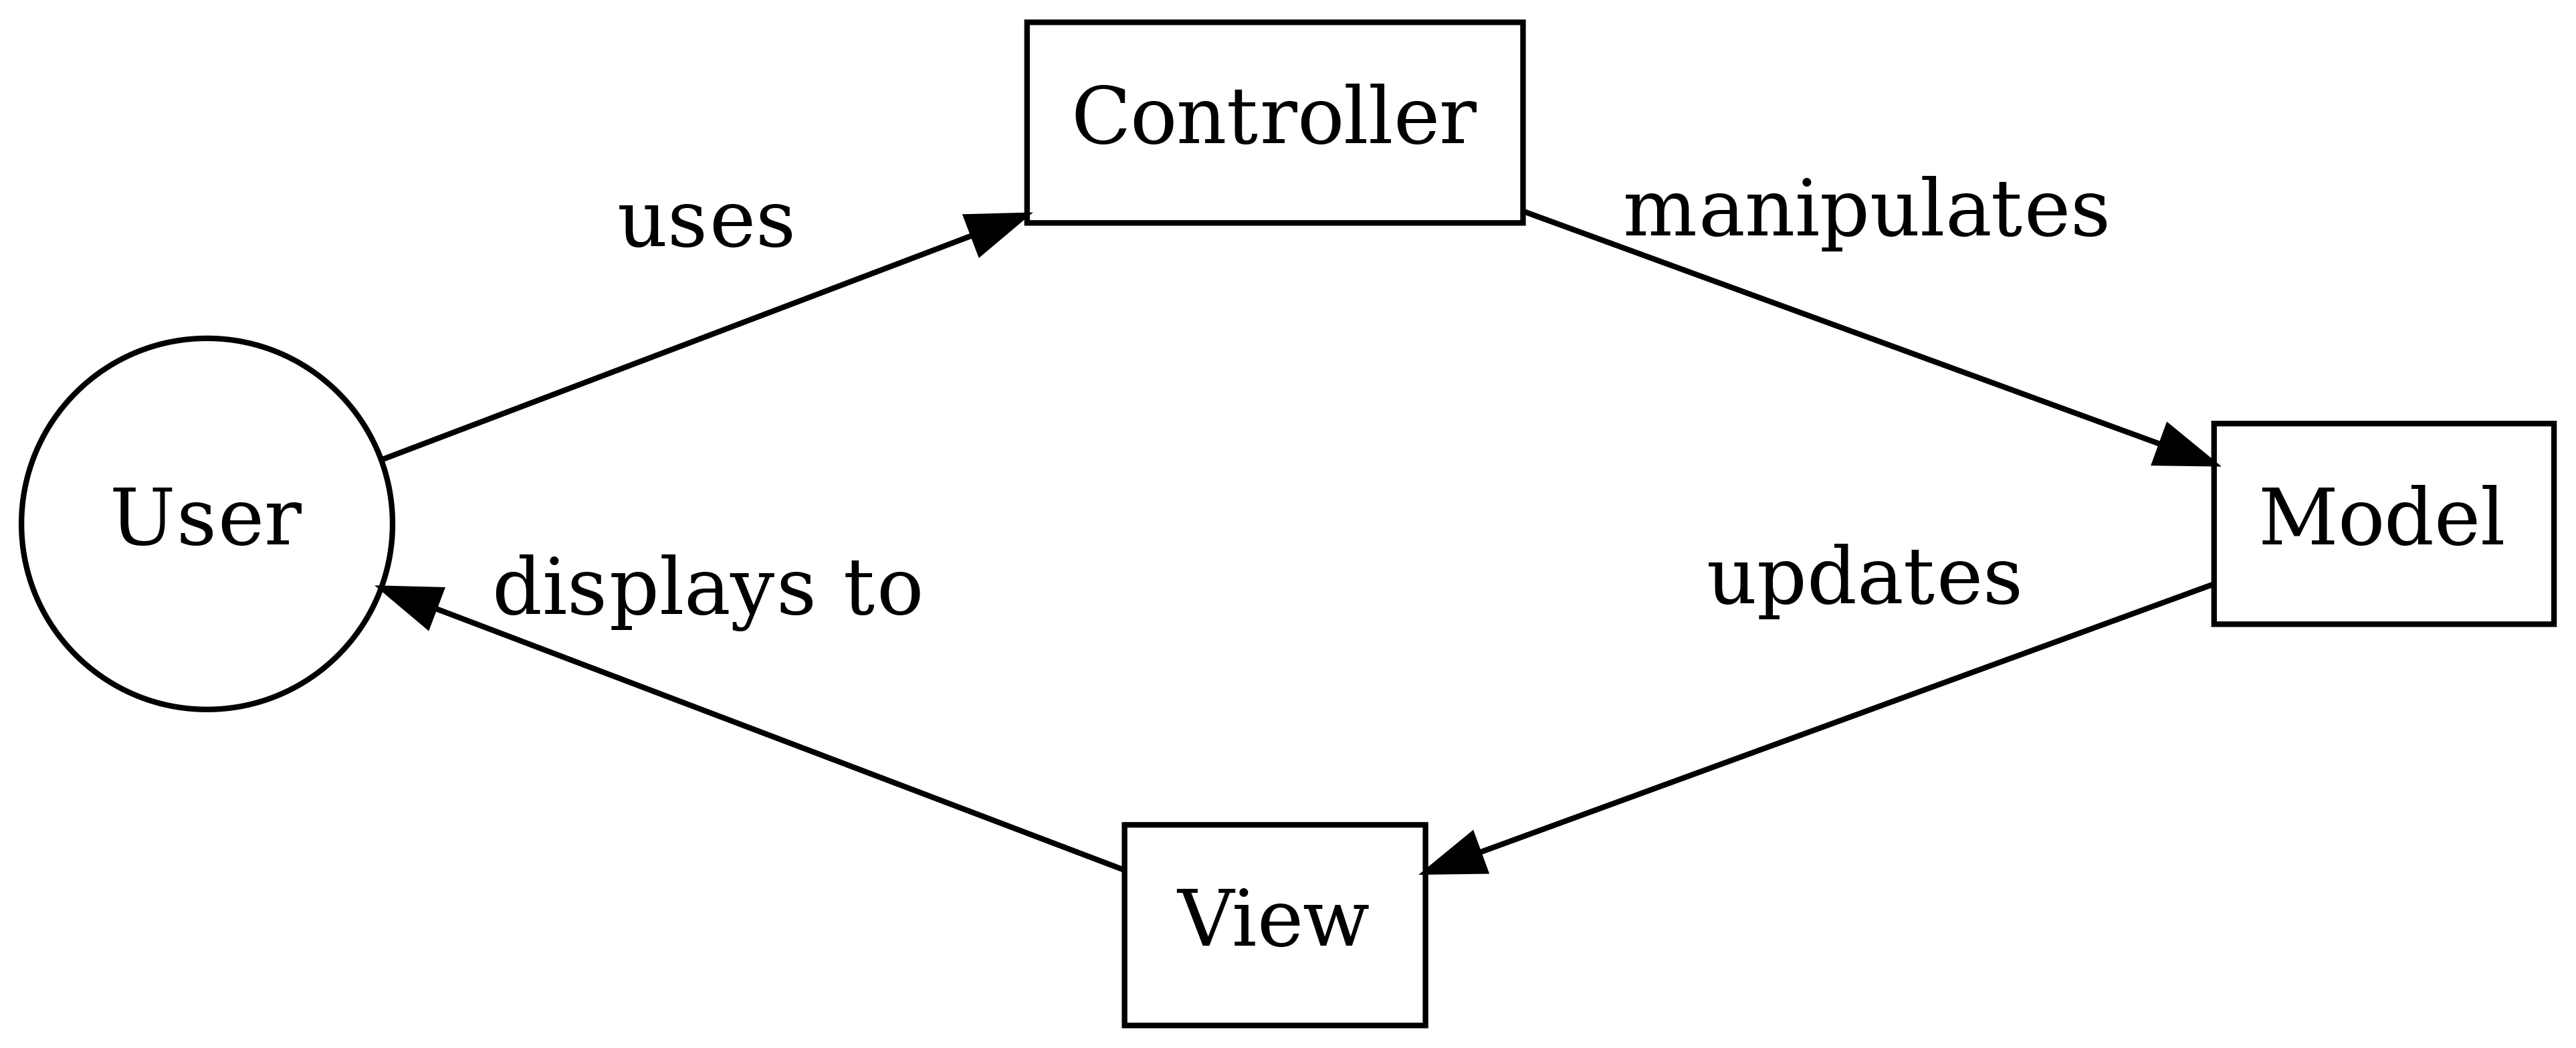
\includegraphics[width=0.8\textwidth]{./img/diagrama-mvc.png}
\end{center}

\tiny
Interacţiunea dintre \texttt{model}, \texttt{view} şi \texttt{controller} în raport cu acţiunile iniţiate de utilizator.
Imagine adaptată după\footnote{\url{https://en.wikipedia.org/wiki/Model-view-controller}}.
\end{frame}
\begin{frame}[label={sec:orga5d2c48},fragile]{Fluxul de lucru}
 \begin{enumerate}
\item Utilizatorul iniţiază o acţiune (click pe buton/request http).
\item \texttt{Controllerul} procesează acţiunea printr-o metodă dedicată.
\item \texttt{Controllerul} notifică \texttt{modelul} existent sau crează unul nou.
\item \texttt{Modelul} îşi schimbă starea (dacă este cazul).
\item \texttt{Viewul} generează interfaţa grafică pe baza modelului.
\item Interfaţa generată aşteaptă alte acţiuni din partea utilizatorului.
\end{enumerate}
\end{frame}
\begin{frame}[label={sec:orgddb36fc},fragile]{Avantaje\footnote{\url{https://en.wikipedia.org/wiki/Model-view-controller}}}
 \begin{itemize}
\item Permite dezvoltarea în paralel; ex. câte un programator per componentă.
\item Grad ridicat de coeziune --- metodele care manipulează acelaşi \texttt{model} pot fi grupate în acelaşi \texttt{controller}; la fel şi \texttt{viewurile}.
\item Grad scăzut de acuplare --- obţinut prin separarea în 3 componente.
\item Componente uşor de modificat.
\item Componentele pot fi testate independent.
\end{itemize}
\end{frame}
\begin{frame}[label={sec:orgb8ab39d}]{Dezavantaje\footnote{\url{https://en.wikipedia.org/wiki/Model-view-controller}}}
\begin{itemize}
\item Mult cod de umplutură.
\item Cod greu de navigat din cauza separării.
\item Necesită disciplină şi exerciţiu --- separarea pe componente nu este intuitivă; în cazuri extreme logica este dispersată în toate cele trei componente.
\end{itemize}
\end{frame}
\section{ASP.NET Core MVC}
\label{sec:org52112b6}
\begin{frame}[label={sec:org9dc2255},fragile]{ASP.NET Core MVC\footnote{\url{https://docs.microsoft.com/en-us/aspnet/core/mvc/overview}}}
 \begin{itemize}
\item Platformă \texttt{open source} de dimensiuni mici.
\item Suportă cele mai noi standarde web.
\item Suportă dezvoltarea în stilul \texttt{TDD}.
\end{itemize}
\end{frame}
\begin{frame}[label={sec:orge268a70},fragile]{Funcţionalităţi suportate}
 \begin{itemize}
\item \texttt{Routing}
\item \texttt{Model binding}
\item Validarea datelor
\item Filtre
\item \texttt{Dependency Injection}
\item Modularizare (\texttt{Areas})
\end{itemize}
\end{frame}
\begin{frame}[label={sec:org12e9749},fragile]{\texttt{Routing}}
 \begin{itemize}
\item Apelează o anumită metodă din \texttt{controller} pe baza unui \texttt{URL} asociat acesteia.
\item Asocierile se fac:
\begin{itemize}
\item pe baza convenţiilor
\item cu atribute dedicate.
\end{itemize}
\end{itemize}
\end{frame}
\begin{frame}[label={sec:orge888305},fragile]{\texttt{Model binding}}
 \begin{itemize}
\item Transformă datele dintr-un \texttt{request} \texttt{http} în instanţe ale tipurilor definite de utilizator.
\item Instanţele rezultate sunt pasate metodelor din controller ca parametri.
\end{itemize}
\end{frame}
\begin{frame}[label={sec:org0db79e9},fragile]{Validarea datelor}
 Validarea se poate face prin:
\begin{itemize}
\item Atribute --- pe client şi server.
\item Metode expuse de biblioteci terţe, ex: \texttt{FluentValidation}\footnote{\url{https://docs.fluentvalidation.net/en/latest/aspnet.html}} --- pe server.
\end{itemize}
\end{frame}
\begin{frame}[label={sec:org8f4be7c}]{Filtre}
Filtrele permit invocarea anumitor metode înainte/după executarea unei anumite părţi din logica aplicaţiei.

Exemple:
\begin{itemize}
\item Restricţionarea accesului la o anumită metodă,
\item Gestiunea erorilor etc.
\end{itemize}
\end{frame}
\begin{frame}[label={sec:orgd1e5733},fragile]{\texttt{Dependency Injection}}
 \texttt{ASP.NET Core MVC} conţine şi un modul propriu de \texttt{Dependency Injection} dar permite şi integrarea de biblioteci terţe specializate (ex. \texttt{AutoFac}\footnote{\url{https://autofaccn.readthedocs.io/en/latest/integration/aspnetcore.html}}) .
\end{frame}
\begin{frame}[label={sec:org0e7a700},fragile]{\texttt{Areas}}
 \begin{itemize}
\item Oferă posibilitatea de a separa aplicaţia în mai multe module.
\item Fiecare modul (\texttt{area}) conţine structura convenţională a unei aplicaţii (\texttt{modele}, \texttt{viewuri}, \texttt{controllere}).
\end{itemize}

Exemple de module:
\begin{itemize}
\item \texttt{Account} --- modificarea datelor utilizatorului; preferinţe etc.
\item \texttt{Accounting} --- facturi, plăţi, bilanţe contabile etc.
\item \texttt{Public} --- toate acţiunile disponibile utilizatorilor neautentificaţi.
\end{itemize}
\end{frame}
\section{Încheiere}
\label{sec:org15f1a3d}
\begin{frame}[label={sec:orga5569b3},fragile]{Recapitulare}
 \begin{itemize}
\item \alert{MVC} este un şablon de proiectare utilizat pentru a decupla interfaţa grafică (\texttt{view}), datele (\texttt{model}) şi logica aplicaţiei (\texttt{controller}).
\item \alert{ASP.NET Core MVC} este o platformă \texttt{open-source} care permite dezvoltarea de aplicaţii Web pe baza convenţiilor asociate şablonului \texttt{MVC}.
\end{itemize}
\end{frame}
\begin{frame}[label={sec:org288bd26}]{Vă mulțumesc!}
\begin{center}
Mulțumesc pentru atenție!
\end{center}
\end{frame}
\end{document}